\documentclass[usenatbib,usegraphicx,letterpaper]{mn2e}
\usepackage[totalwidth=480pt,totalheight=680pt]{geometry}

\usepackage{lmodern}

\usepackage{amsmath}
\usepackage{amstext}
\usepackage{amssymb}
\usepackage{yfonts}

\usepackage{epsfig}
\usepackage{graphicx}
\usepackage{color}

\usepackage[lowtilde]{url}
\usepackage{hyperref}

\bibliographystyle{mn2e}

%-------- journals
\newcommand{\araa}{ARAA~}
\newcommand{\apj}{ApJ~}
\newcommand{\apjl}{ApJL~}
\newcommand{\apjs}{ApJS~}
\newcommand{\mnras}{MNRAS~}
\newcommand{\nat}{Nature~}
\newcommand{\physrep}{Phys. Rep.~}
\newcommand{\aj}{AJ~}
\newcommand{\pasp}{ASP~}

%%%% Misc %%%
\newcommand{\beq}{\begin{equation}}
\newcommand{\eeq}{\end{equation}}
\newcommand{\beqray}{\begin{eqnarray}}
\newcommand{\eeqray}{\end{eqnarray}}

\newcommand{\ben}{\begin{enumerate}}
\newcommand{\een}{\end{enumerate}}
\newcommand{\bit}{\begin{itemize}}
\newcommand{\eit}{\end{itemize}}

%%%%%%%%  galaxy properties  %%%%%%%%
\newcommand{\rhalf}{R_{1/2}}
\newcommand{\rhalfdisk}{R_{1/2}^{\rm disk}}
\newcommand{\rhalfbulge}{R_{1/2}^{\rm bulge}}
\newcommand{\adisk}{A_{\rm disk}}
\newcommand{\abulge}{A_{\rm bulge}}
\newcommand{\alphadisk}{\alpha_{\rm disk}}
\newcommand{\alphabulge}{\alpha_{\rm bulge}}
\newcommand{\sigmarhalf}{\sigma_{\rm R_{1/2}}}
\newcommand{\bt}{{\rm B/T}}
\newcommand{\mstar}{M_{\ast}}
\newcommand{\ssfr}{{\rm sSFR}}
\newcommand{\sfr}{{\rm SFR}}

%%%%%%%%  halo properties  %%%%%%%%
\newcommand{\halospin}{\lambda_{\rm halo}}
\newcommand{\mvir}{M_{\rm vir}}
\newcommand{\macc}{M_{\rm acc}}
\newcommand{\mpeak}{M_{\rm peak}}
\newcommand{\zpeak}{z_{M_{\rm peak}}}
\newcommand{\mhalo}{M_{\rm halo}}
\newcommand{\mhost}{M_{\rm host}}
\newcommand{\rvir}{R_{\rm vir}}
\newcommand{\rmpeak}{R_{\rm M_{peak}}}
\newcommand{\vmaxmpeak}{V_{\rm peak}}
\newcommand{\vmax}{V_{\rm max}}
\newcommand{\rspeak}{{R_{\rm s,}}_{\rm M_{peak}}}


%%%%%%%%  cosmology  %%%%%%%%
\newcommand{\lcdm}{\Lambda{\rm CDM}}

%%%%%%%%  observations  %%%%%%%%
\newcommand{\rproj}{r_{\rm p}}
\newcommand{\wproj}{w_{\rm p}}
\newcommand{\wplarge}{w_{\rm p}^{\rm large}}
\newcommand{\wpsmall}{w_{\rm p}^{\rm small}}
\newcommand{\wpall}{w_{\rm p}^{\rm all}}

\newcommand{\median}[2]{\langle{#1}\vert{#2}\rangle_{\rm median}}

%%%%%%%%  units  %%%%%%%%
\newcommand{\kpc}{{\rm kpc}}
\newcommand{\mpc}{{\rm Mpc}}
\newcommand{\msun}{M_\odot}
\newcommand{\kms}{{\rm km/s}}

%%%%%%%%%%%%%%%%%%%%%%%%%%%%%%%%
%%%%%%%%%%%%%%%%%%%%%%%%%%%%%%%%


\usepackage{epsfig}  \usepackage{graphicx}   \usepackage{rotating}

\begin{document}

\title[The Relative Sizes of Centrals and Satellites]
{Clustering Constraints on the Relative Sizes of Central and Satellite Galaxies}


\author[Hearin, Behroozi, Kravtsov \& Moster]{
Andrew Hearin$^{1}$, Peter Behroozi$^{2}$, Andrey Kravtsov$^{3}$, Benjamin Moster$^{4}$\\
$^{1}$Argonne National Laboratory, Argonne, IL, USA 60439, USA\\
$^{2}$Department of Physics, University of Arizona, 1118 E 4th St, Tucson, AZ 85721 USA\\
$^{3}$Department of Astronomy \& Astrophysics, The University of Chicago, Chicago, IL 60637 USA\\
$^{4}$Universit{\"a}ts-Sternwarte, Ludwig-Maximilians-Universit{\"a}t M{\"u}nchen, Scheinerstr. 1, 81679 M{\"u}nchen, Germany
}

\maketitle

\begin{abstract}
We place empirical constraints on the connection between dark matter halos and galaxy half-light radii, $\rhalf.$ Low-redshift SDSS measurements show that smaller galaxies cluster much more strongly than larger galaxies at fixed stellar mass. Using {\tt Halotools} to forward model the observations, we find that the clustering signal generically requires satellite galaxies to be smaller than central galaxies of the same halo mass. We present a simple empirical model consistent with the clustering results, in which galaxy size is proportional to halo virial radius at the time of peak halo mass. We use this model to predict how galaxy lensing, $\Delta\Sigma,$ should depend on $\rhalf$ for $\mstar-$complete samples. Other simple empirical models fail the clustering test, such as models in which galaxy size is related to stellar mass alone; these failures persist even when accounting for possible effects from satellite stripping and orphan galaxies. Our results suggest that the relative size of centrals and satellites is predetermined at the time of satellite infall, and that a remarkably simple galaxy--halo scaling relation emerges from the complex physics regulating galaxy size.
\end{abstract}

\section{Introduction}
\label{sec:intro}

In the $\lcdm$ framework of cosmological structure formation, galaxies form at the centers of dark matter halos. Highly complex and nonlinear baryonic processes regulate galaxy formation, and the quest for a fine-grained understanding of these processes is one of the chief goals of theoretical astrophysics today.

Observationally, many properties of observed galaxies exhibit remarkably tight scaling relations. Among the most fundamental of these relations is the strong correlation between galaxy size and stellar mass and luminosity. The scaling of galaxy size with galaxy mass is well-measured in the local Universe \citep{shen_etal03,guo_etal09,huang_etal13,zhang_yang17} and at high-redshift \citep{trujillo_etal04,vanderwel_etal14,kawamata_etal15,shibuya_etal15,huertas_company_etal13a,lange_etal15,huang_etal17}.

These well-measured scaling relations are challenging to faithfully recover using ab initio galaxy formation methods such as hydrodynamical simulations and semi-analytic models, and provide useful boundary conditions for the calibration of such modeling efforts \citep{khochfar_silk06,dutton_etal10,hopkins_etal10a,bottrell_etal17b}. The precision cosmology program also depends critically on accurate modeling of galaxies, so that cosmological parameter inference can be confidently conducted without undue interference from uncertainty in baryonic physics \citep{LSST_science,LSST_galaxies}.



\section{Data and Simulations}
\label{sec:data}

Our galaxy sample comes from the catalog of SDSS galaxy profile decompositions provided by \citet{meert_etal15}. This catalog is based on Data Release 10 of the Sloan Digital Sky Survey \citep[SDSS,][]{ahn_etal14}, with improvements to the photometry pipeline and light profile fitting methods \citep{vikram_etal10,bernardi_etal13,bernardi_etal14,meert_etal13}. In the version of this catalog that we use, two-dimensional $r-$band profiles were fit with a two-component de Vaucouleurs + exponential profile to determine the half-light radius $\rhalf.$ We use stellar mass measurements made available through the MPA-JHU catalog \citep{kauffmann_etal03,brinchmann_etal04}, allowing us to define volume-limited samples of galaxies according to the same completeness cuts used in \citet{behroozi_etal15} (see Figure 2).

We calculate two-point clustering $\wproj$ of our SDSS galaxy sample using line-of-sight projection of $\pi_{\rm max}=20\mpc$ using the {\tt correl} program in {\tt UniverseMachine}. {\color{red} PSB: Please fill in details about {\tt correl} here}.

As the bedrock of our modeling, we use the publicly available\footnote{\url{http://www.slac.stanford.edu/~behroozi/BPlanck\_Hlists}} catalog of {\tt Rockstar} subhalos identified at $z=0$ in the Bolshoi-Planck simulation \citep{klypin_etal11,behroozi12_rockstar,behroozi12_consistent_trees,riebe_etal13,rodriguez_puebla16_bolplanck}. As described in \S\ref{subsec:sham}, we will use traditional abundance matching to connect stellar mass $\mstar$ with subhalo peak mass $\mpeak.$ To address issues related to subhalo incompleteness \citep{guo_white13}, we supplement the Bolshoi-Planck subhalo catalog with {\em all} subhalos that were ever identified by {\tt Rockstar}, including those that no longer appear in the standard catalog as subhalos that survive to $z=0.$ We describe our treatment of these ``orphan" subhalos in the Appendix.

For mock galaxies, to compute galaxy clustering we employ the distant observer approximation by treating the simulation $z-$axis as the line-of-sight. We compute $\wproj$ using the {\tt mock\_observables.wp} function in {\tt Halotools}, which is a python implementation of the algorithm in the {\tt Corrfunc} C library \citep{sinha_etal17}.

All numerical values of $\rhalf$ will be quoted in physical $\kpc,$ and all values of $\mstar$ and $\mhalo$ in $\msun,$ assuming $H_0=67.8~\kms\equiv100h~\kms,$ the best-fit value from \citet{planck15}. To scale stellar masses to ``$h=1$ units" \citep{croton13}, our numerically quoted values for $\mstar$ should be multiplied by a factor of $h^2,$ while our halo masses and distances should be multiplied by a factor of $h.$

\subsection{Classifying large vs. small galaxies}
\label{subsec:sizedef}

Because galaxy clustering has well-known dependence upon $\mstar$ that is not the subject of this work, we wish to remove this influence and focus purely on the relationship between $\rhalf$ and $\wproj(\rproj).$ To do so, we determine the value $\median{\rhalf}{\mstar}$ by computing a sliding median of $\rhalf,$ calculated using a window of width $N_{\rm gal}=1000.$ Each galaxy is categorized as either ``large" or ``small" according to whether it is above or below the median value appropriate for its stellar mass. We note that this is directly analogous to the common convention for studying the properties of ``red" vs. ``blue" galaxies, in which the two subsamples are divided by a $\mstar-$ or luminosity-dependent green valley cut \citep[e.g.,][]{vdB_etal08,zehavi_etal11}. 

Using this technique, for any $\mstar-$threshold sample, the stellar mass function of the ``large" and ``small" subsamples are identical. We illustrate this for the particular case of $\mstar>10^{10.25}\msun$ in left panel of Figure~\ref{fig:sizedefinition}, which shows histograms of stellar mass for the two subsamples. The right panel of Figure~\ref{fig:sizedefinition} compares histograms of their size distributions, which partially overlap due to the variation in $\median{\rhalf}{\mstar}$ across the $\mstar-$ range of the threshold sample. 


%---------------------------------------------------------------------------------------------------
\begin{figure}
\centering
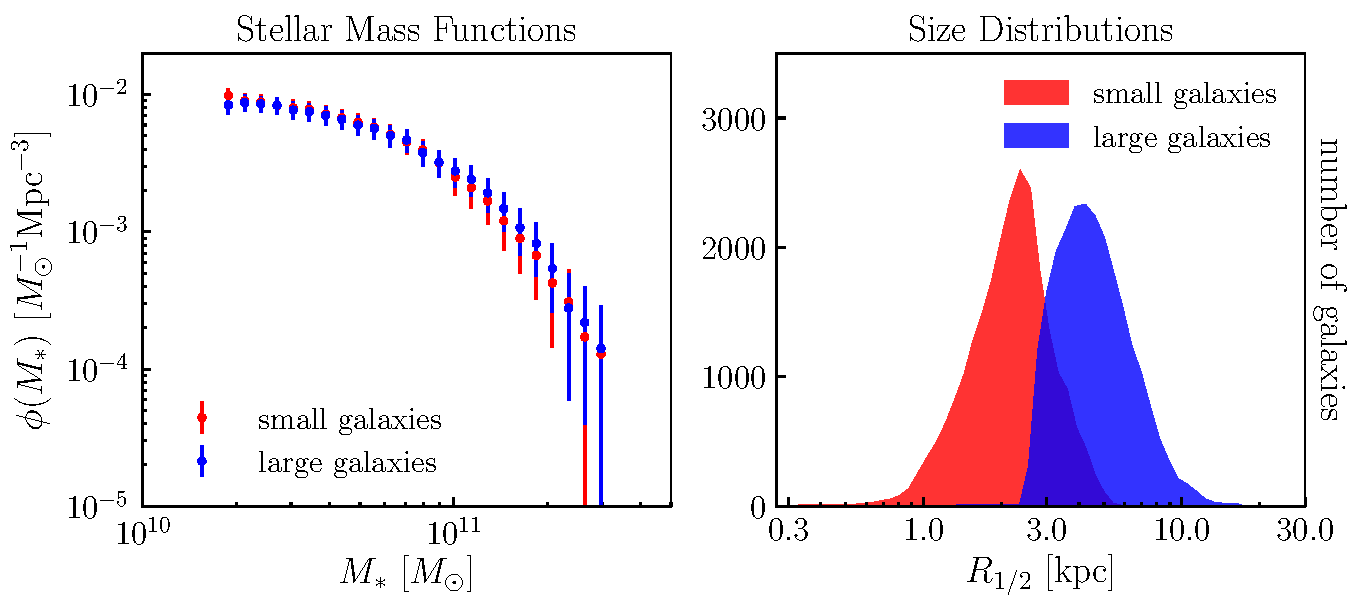
\includegraphics[width=8cm]{FIGS/sdss_small_large_sample_definitions.pdf}
\caption{
{\bf Definition of ``small" and ``large" galaxies.} For a volume-limited SDSS galaxy sample defined by $M_{\ast}>10^{10.25}M_{\odot},$ we visually demonstrate how we classify galaxies into ``small" and ``large" subsamples. As described in detail in \S\ref{subsec:sizedef}, we compute the median value $\median{\rhalf}{\mstar}$ using a sliding window with a width of $1000$ galaxies at each value of $\mstar.$ The {\em left panel} shows a histogram of the stellar masses, confirming that our method yields identical stellar mass functions for the two subsamples. The {\em right panel} shows histograms of $\rhalf$ for the two subsamples, which partially overlap due to the finite range of $\mstar$ in the volume-limited sample.
}
\label{fig:sizedefinition}
\end{figure}
%-----------------------------------------------------------------------------------------------------

\section{Galaxy-Halo Model}
\label{sec:model}

\subsection{Abundance Matching}
\label{subsec:sham}

We map $\mstar$ onto subhalos using deconvolution abundance matching on the orphan-supplemented Bolshoi-Planck subhalo catalog, as described in detail in the Appendix. Briefly, our abundance matching prescription is based $\mpeak,$ the largest value of $\mvir$ ever attained along the main progenitor branch of the subhalo.

%---------------------------------------------------------------------------------------------------
\begin{figure}
\centering
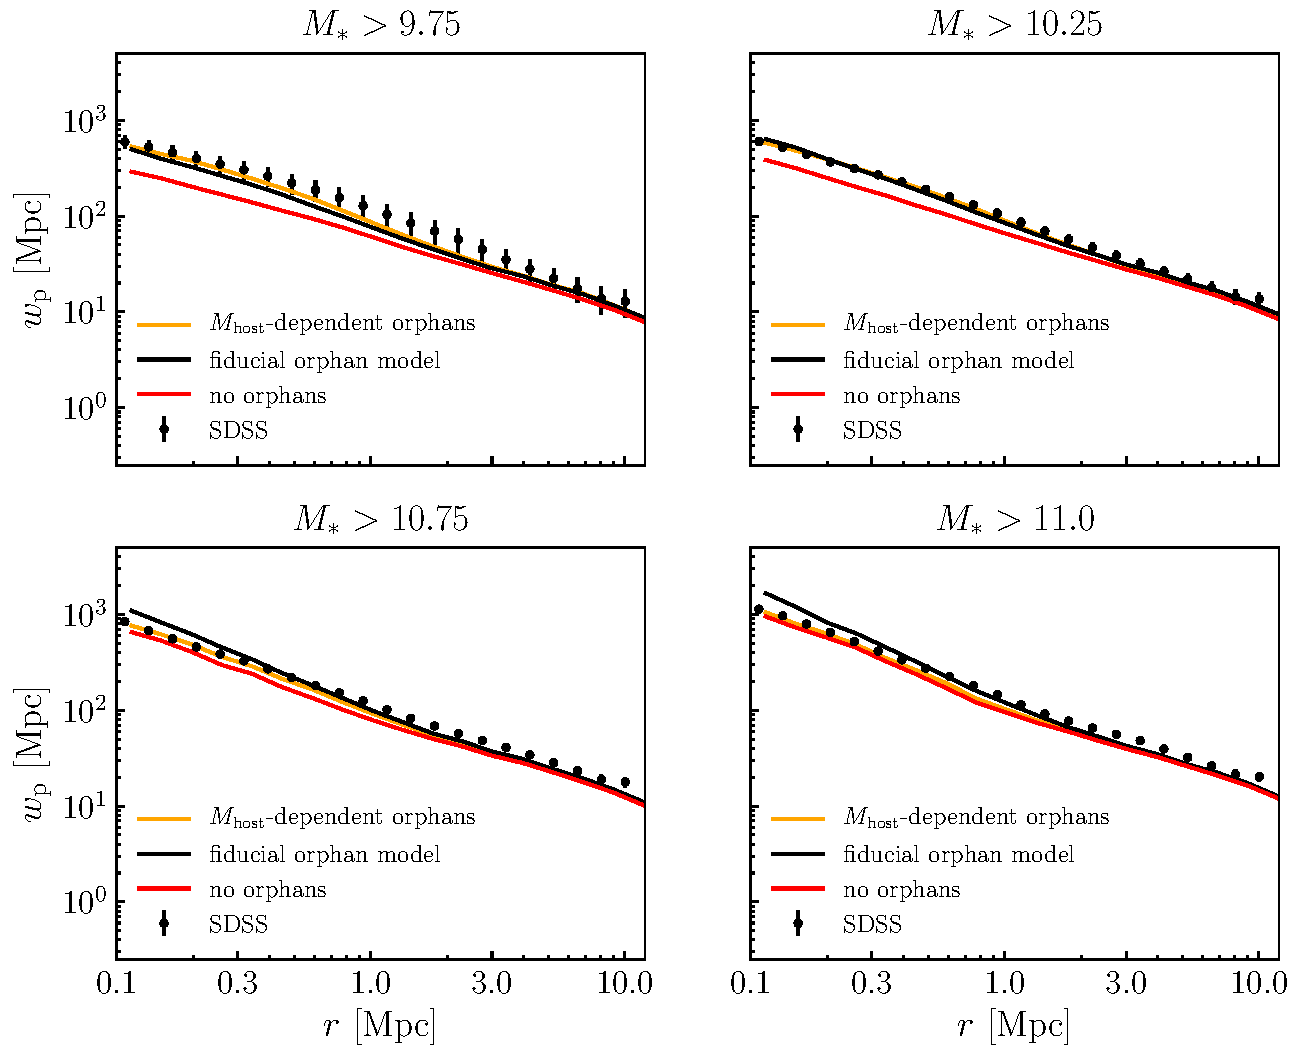
\includegraphics[width=8cm]{FIGS/baseline_sham_orphans.pdf}
\caption{
{\bf SHAM + orphan clustering predictions.}
Using the abundance matching methods described in \S\ref{subsec:smhm}, we compare the projected clustering of mock vs. SDSS galaxies. Each panel shows the comparison for a volume-limited sample defined by a different $\mstar-$threshold. Black points with error bars show SDSS measurements; solid red (black) curves show the abundance matching prediction including (excluding) the effect of orphan subhalos (see Appendix A). Including orphans mitigates the discrepancy in the clustering predicted by traditional, $\mpeak-$based SHAM based, though mild tension remains for $\mstar\gtrsim10^{10.75}\msun.$
}
\label{fig:baseline_sham_clustering}
\end{figure}
%-----------------------------------------------------------------------------------------------------

\subsection{Galaxy size models}
\label{subsec:model}

In \S\ref{sec:results}, we calculate predictions for the $\rhalf-$dependence of galaxy clustering for several different kinds of empirical models, described in turn below.


\subsubsection{$\mstar-$based model}
\label{subsubsec:mstaronlymodel}

In the first class of models we explore, we suppose that stellar mass $\mstar$ is the statistical regulator of $\rhalf,$ so that galaxy sizes are drawn from a log-normal distribution centered at $\median{\rhalf}{\mstar}.$ To implement this model, for simplicity we directly tabulate $\median{\rhalf}{\mstar}$ directly from the data, rather than pursue a parametric form \citep[see, e.g.,][]{zhang_yang17}.

\subsubsection{$\rvir-$based model}
\label{subsubsec:rvirmodel}

Motivated by \citet{kravtsov13}, we explore a model in which $\rhalf$ is linearly proportional to halo virial radius:
\beq
\label{eq:fiducial_model}
\rhalf = 0.01\rvir
\eeq
For the virial radius of halos and subhalos, we use $\rmpeak,$ the value of $\rvir$ in physical units of $\kpc$ measured at the time of peak subhalo mass, defined by
\beq
\mpeak\equiv\frac{4\pi}{3}\rmpeak^{3}\Delta_{\rm vir}(\zpeak)\rho_{\rm m}(\zpeak),
\eeq
where for $\Delta_{\rm vir}(\zpeak)$ we use the fitting function to the ``virial" definition used in \citet{bryan_norman98}. For the model we refer to as the ``$\rvir-$based model", we add uncorrelated log-normal scatter of $\sigmarhalf=0.2$ dex to generate a Monto Carlo realization of the model population.

\subsubsection{$\mstar-$stripping model}
\label{subsubsec:strippingmodel}

As we will show in \S\ref{sec:results}, the chief ingredient needed to recover the observed clustering properties of galaxies is that satellites need to be smaller than centrals of comparable halo mass. Thus it is natural to consider a class of models in which stellar mass is stripped from satellite galaxies after infall.
 %satellites lose stellar mass in a way that mimics what is seen in high-resolution hydrodynamical simulations. 

The basis of this class of models is the fitting function presented in \citet{smith_etal16}, which was calibrated by studying stellar mass loss in a suite of high-resolution hydrodynamical simulations. In this model, $f_{\ast}$ quantifies the fraction of stellar mass lost as a function of $f_{\rm DM},$ the amount of dark matter that has been stripped since infall:

\beq
f_{\ast} = 1 - \exp(-14.2f_{\rm DM})
\eeq
For $f_{\rm DM}$ we use the ratio of present-day subhalo mass divided by the peak mass, $M_{\rm vir}/M_{\rm peak}.$ If we denote the post-stripping stellar mass as $M_{\ast}',$ then we have $M_{\ast}'\equiv f_{\ast}M_{\ast},$ where $M_{\ast}$ is given by Eq.~\ref{eq:smhm}. We then calculate the post-stripping radius by interpolating $\langle\rhalf'\vert\mstar'\rangle$ directly from SDSS data.

\section{Results}
\label{sec:results}

\subsection{Size-Mass Scaling Relation}
\label{subsec:one_point_function}

In Figure \ref{fig:scatter_plot} we show the scaling of galaxy size $\rhalf$ with $\mstar.$ The black curve enveloped by the gray bands shows the scaling relation for SDSS galaxies, while the blue curve shows the median relation  $\median{\rhalf}{\mstar}$ implied by the $\rvir-$based model described in \S\ref{subsubsec:rvirmodel}. This figure shows that models in which $\rhalf\propto\rvir$ can naturally give rise to the characteristic curvature in the $\rhalf-\mstar$ relation, confirming the results in \citet{kravtsov13} in a forward modeling context.

%---------------------------------------------------------------------------------------------------
\begin{figure}
\centering
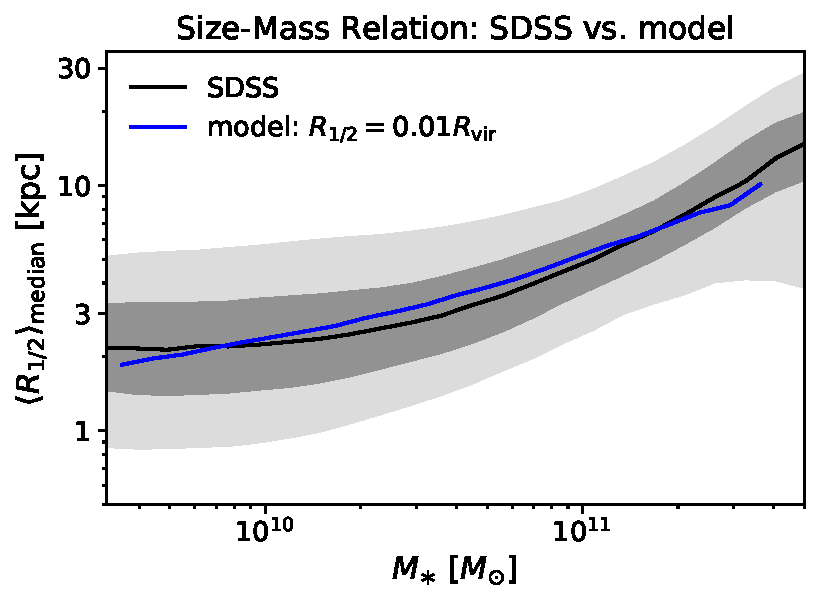
\includegraphics[width=8cm]{FIGS/rvir_only_rhalf_vs_mstar_sham_model.pdf}
\caption{
The black curve shows the median size-mass relation of SDSS galaxies as measured in \citet{meert_etal15}. The two gray bands enveloping the black curve show the $50\%$ and $90\%$ percentile regions. The blue curve shows $\rvir-$based model in which $\median{\rhalf}{\rvir}=0.01\rvir.$ This figure confirms that a linear relationship between $\rvir$ and $\rhalf,$ convolved against the nonlinear relationships between $\rvir, \mhalo$ and $\mstar,$  predicts the characteristic curvature in the relation $\median{\rhalf}{\mstar}$ over a wide range in mass.
}
\label{fig:scatter_plot}
\end{figure}
%-----------------------------------------------------------------------------------------------------

\subsection{Size-Dependent Clustering}
\label{subsec:clustering_results}

In Figure~\ref{fig:rvir_only_clustering_absolute}, we present new measurements of the $\rhalf-$dependence of projected galaxy clustering, $\wproj(\rproj).$ We measure $\wproj(\rproj)$ separately for large and small subsamples for four different $\mstar$ thresholds, $\mstar>10^{9.75}\msun,$ $\mstar>10^{10.25}\msun,$ $\mstar>10^{10.75}\msun,$ and $\mstar>10^{11}\msun.$ For each threshold, we split the galaxies into ``large" and ``small" subsamples; as described in \S\ref{subsec:sizedef} and illustrated in Figure \ref{fig:sizedefinition}, our size-based selection is defined so that the subsamples have identical stellar mass functions. Red points with jackknife-estimated error bars show SDSS measurements of $\wproj(\rproj)$ for small galaxy samples, blue points show the same for large galaxies. Solid curves show $\wproj$ as predicted by the $\rvir-$based model described in \S\ref{subsubsec:rvirmodel}. 

The salient feature of these clustering measurements is that small galaxies cluster more strongly than large galaxies of the same stellar mass. This feature also holds true for galaxies predicted by the $\rvir-$based model. This result may be surprising, since $\rhalf\propto\rvir,$ halo mass $\rvir\propto\mhalo^{1/3},$ and clustering strength increases with $\mvir.$ Based on this simple argument, one would expect that large galaxies would be the more strongly clustered. We provide a resolution to this conundrum in \S\ref{subsec:censat_sizes}; before doing so, we first examine the clustering test of the $\rvir-$based model in more detail.

As shown in Figure \ref{fig:baseline_sham_clustering}, the abundance matching prediction for $\wproj(\rproj)$ exhibits tension with SDSS observations at the $10-20\%$ level, particularly for $\mstar\gtrsim10^{10.75}\msun.$ This tension is inherited by our $\rvir-$based model for size, which is the subject of this work, and so we wish to compare our size models to data in such a way that minimizes the role played by the underlying stellar-to-halo-mass relation. We accomplish this using {\em the $\rhalf$ clustering ratios,} described below. 

For each volume-limited $\mstar-$threshold sample, we additionally measure $\wproj(\rproj)$ {\em without} splitting on size, giving us measurements $\wpall, \wplarge,$ and $\wpsmall$ for each threshold sample. This allows us to compute the ratio $(\wplarge-\wpsmall)/\wpall,$ which we refer to as {\em the $\rhalf$ clustering ratio}, denoted as $\delta_{\rhalf}(\wproj).$ For example, a clustering ratio of $-0.5$ corresponds to small galaxies being $50\%$ more strongly clustered than large galaxies of the same stellar mass. These ratios are the measurements appearing on the y-axis in each panel of Figure \ref{fig:clustering_ratio_upshot}. 

The points and curves in Figure \ref{fig:clustering_ratio_upshot} are all negative: small galaxies cluster more strongly relative to large. This presentation of the measurement makes plain that the underlying signal of $\rhalf-$dependent clustering is strongest for samples with smaller stellar mass; as $\mstar$ increases, the signal weakens and nearly vanishes for $\mstar\gtrsim10^{11}\msun.$ Strikingly, the $\rvir-$based model exhibits this $\mstar-$dependent behavior, as well as the scale-dependence of the observed clustering signal at each $\mstar.$ As described in \S\ref{subsec:censat_sizes} below, we attribute the success of this prediction to the relative sizes of central vs. satellite galaxies. 

%---------------------------------------------------------------------------------------------------
\begin{figure*}
\centering
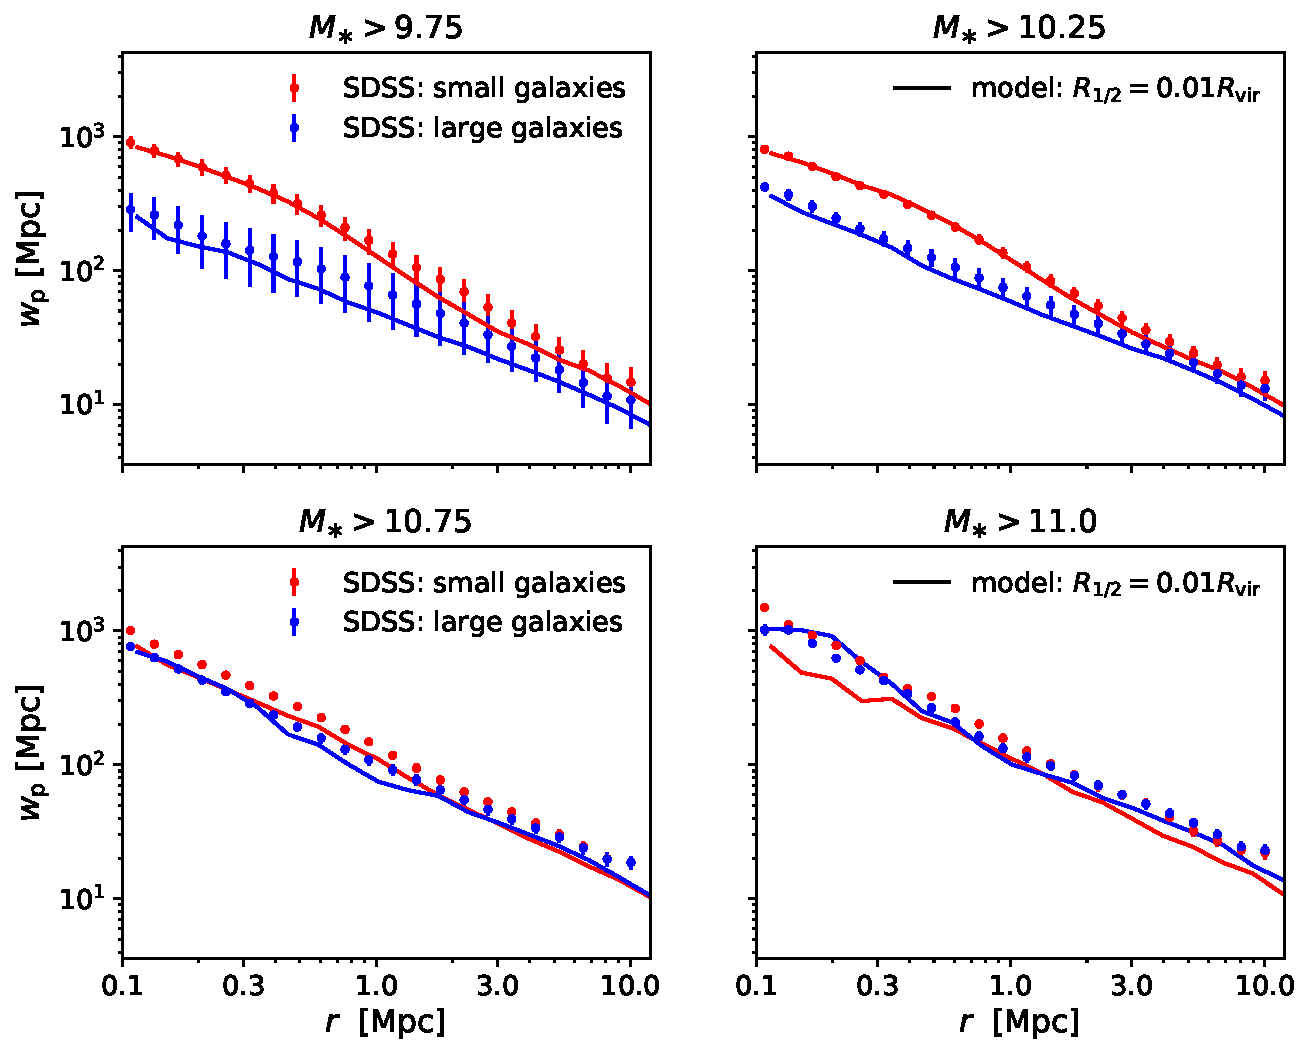
\includegraphics[width=12cm]{FIGS/rvir_only_wp_large_small_absolute.pdf}
\caption{
{\bf $\rhalf-$dependence of galaxy clustering.}
Red and blue points with error bars show our SDSS measurements of the clustering of small and large galaxies, respectively. For each volume-limited sample of $\mstar-$complete galaxies, the small and large subsamples have identical stellar mass functions, as shown in Figure \ref{fig:sizedefinition}. Small galaxies cluster much more strongly relative to large galaxies of the same stellar mass. Solid curves show the clustering predictions of the $\rvir-$based model described in \S\ref{subsubsec:rvirmodel}. The $\rvir-$based model inherits the shortcoming of ordinary abundance matching at $\mstar\gtrsim10^{10.75}\msun,$ although the model faithfully captures the {\em relative} clustering of small vs. large galaxies, as shown in Figure \ref{fig:clustering_ratio_upshot}.
}
\label{fig:rvir_only_clustering_absolute}
\end{figure*}
%-----------------------------------------------------------------------------------------------------

%---------------------------------------------------------------------------------------------------
\begin{figure*}
\centering
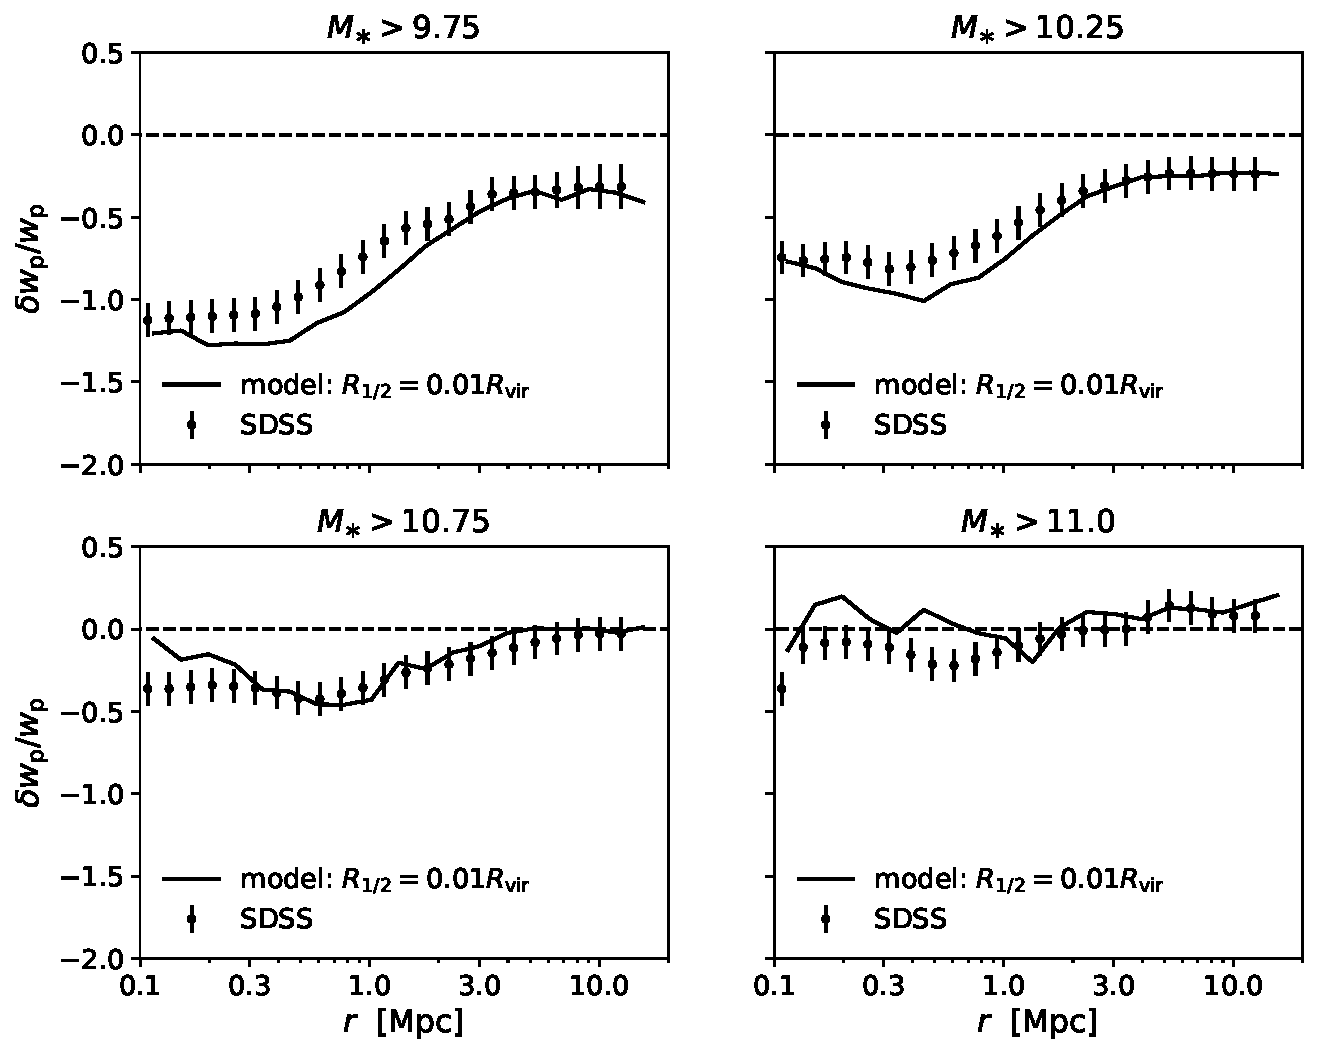
\includegraphics[width=12cm]{FIGS/rvir_only_wp_ratios.pdf}
\caption{
{\bf $\rhalf-$dependence of galaxy clustering: clustering ratios.}
Closely related to Figure \ref{fig:rvir_only_clustering_absolute}, the y-axes show {\em clustering strength ratios,} defined as $(w_{\rm p}^{\rm large} - w_{\rm p}^{\rm small})/w_{\rm p}^{\rm all}.$ Thus a y-axis value of $-0.5$ corresponds to small galaxies being $50\%$ more strongly clustered than large galaxies of the same stellar mass. Solid curves show the clustering ratio predictions of the $\rvir-$based model described in \S\ref{subsubsec:rvirmodel}. Normalizing the measurements and predictions by $w_{\rm p}^{\rm all}$ scales away the shortcoming of ordinary abundance matching at high stellar mass (see Figure \ref{fig:baseline_sham_clustering}), highlighting the successful prediction of the $\rvir-$based model for the $\rhalf-$dependence of galaxy clustering.
}
\label{fig:clustering_ratio_upshot}
\end{figure*}
%-----------------------------------------------------------------------------------------------------

\subsection{Central vs. Satellite Sizes}
\label{subsec:censat_sizes}

The clustering measurements shown in the previous section present a puzzle. The modeling assumption $\rhalf\propto\rvir$ predicts size-dependent galaxy clustering that is in quite good agreement with observations, particularly considering the simplicity of the model. Yet, small galaxies cluster more strongly relative to large, which seems at odds with naive expectations based on halo mass, since $\rvir\propto\mvir.$ A straightforward resolution to this puzzle is shown in Figure \ref{fig:censatsizehist}, which compares the $\rhalf$ distributions of central, satellite, and splashback galaxies with the same halo mass $\mhalo\equiv\mpeak\approx10^{12}\msun.$ A ``splashback central"  is defined as a present-day central that used to be a satellite, i.e., its main progenitor halo passed inside the virial radius of a larger halo at some point in its past history. On the other hand, we define a ``true central" as a galaxy that has never been a satellite.

%---------------------------------------------------------------------------------------------------
\begin{figure}
\centering
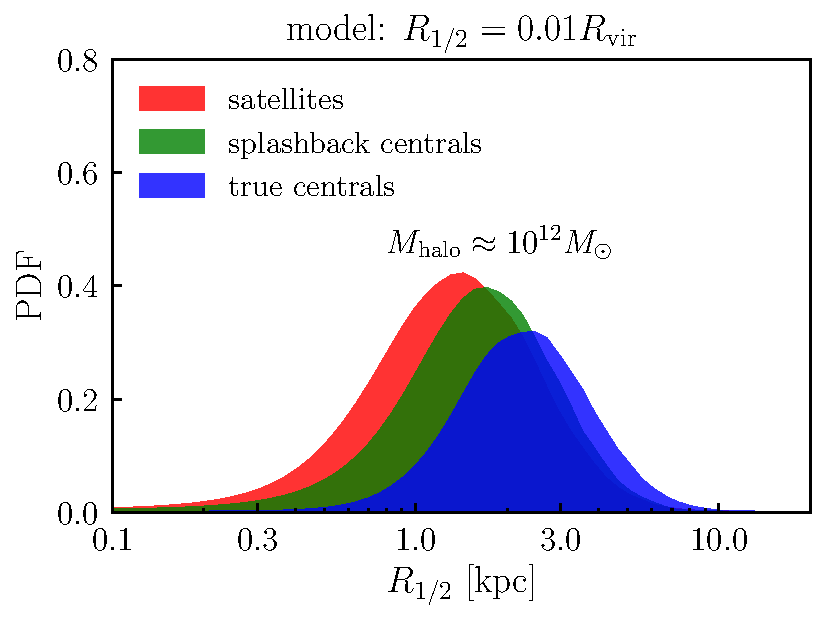
\includegraphics[width=8cm]{FIGS/rvir_only_cen_sat_sizes.pdf}
\caption{
{\bf Relative sizes of centrals and satellites.}
In a narrow bin of halo mass $\mhalo\equiv\mpeak\approx10^{12}\msun,$ we show the distribution of model galaxy sizes for different subpopulations galaxies, as predicted by the $\rvir-$based model. The red histogram shows the sizes of satellites; the blue histogram shows host halos that have never passed inside the virial radius of a larger halo (``true centrals"); the green histogram host halos that were subhalos inside a larger at some point in their past history (``splashback centrals"). In the $\rvir-$based model, galaxy size is set by the {\em physical} size of the virial radius at the time the halo attains its peak mass, naturally resulting in smaller sizes for satellites and splashback centrals relative to true centrals of the same $\mhalo.$
}
\label{fig:censatsizehist}
\end{figure}
%-----------------------------------------------------------------------------------------------------

In the $\rvir-$based model, satellite and splashback galaxies are smaller than centrals of the same halo mass due to the physical size of their halo being smaller at earlier times $\zpeak.$ There are two distinct reasons why this feature results in small galaxies being more strongly clustered relative to larger galaxies of the same mass. First and foremost, satellite galaxies statistically occupy higher mass host halos that are more strongly clustered. So in models where satellites are smaller than centrals, at fixed $\mstar$ the ``small" subsample will naturally have a higher satellite fraction, boosting the clustering of small galaxies relative to large of the same stellar mass. Second, at fixed mass, halos of $L_\ast$ galaxies that form earlier are more strongly clustered, a phenomenon commonly known as {\em halo assembly bias}. Splashback halos are typically earlier-forming than true centrals, and so models where splashback halos host smaller-than-average galaxies will naturally predict smaller galaxies being the more strongly clustered. We highlight this point in section \ref{subsec:orphan_stripping} below by testing predictions for $\mstar-$based models that do not possess central vs. satellite size differences. 

\subsection{Failure of $\mstar-$based Models}
\label{subsec:orphan_stripping}

The green curves in Figure~\ref{fig:mstarmodelclustering} test the clustering predictions of the $\mstar-$based model described in \S\ref{subsubsec:mstaronlymodel}. In this model, $\rhalf$ is a log-normal distribution centered at $\median{\rhalf}{\mstar}.$ By construction, this model predicts no dependence at all of galaxy clustering upon $\rhalf$ at fixed $\mstar,$ even though the observed one-point distributions are recovered exactly. 

The reason for the null signal of the purely $\mstar-$based model is simply that the scatter of $\rhalf$ about $\median{\rhalf}{\mstar}$ is uncorrelated with any other property. This is in contrast to the $\rvir-$based model, which correlates the scatter with host halo mass and as well as subhalo assembly. The purely $\mstar-$based model gives us a useful starting point to test simple alternative hypotheses for how the scatter may be correlated with large-scale structure. This is the motivation behind the $\mstar+$stripping model described in \S\ref{subsubsec:strippingmodel}. In this alternative model, satellites have smaller sizes than centrals of the same $\mstar$ due to post-infall stripping, where the amount of stripping has been calibrated to the satellite mass loss seen in high-resolution hydrodynamical simulations. 

The treatment of stellar mass loss in this model naturally results in an enhancement of size differences between satellites and centrals. As shown by the purple curves in Figure \ref{fig:mstarmodelclustering}, these central/satellite differences impact $\rhalf-$dependent clustering in the expected manner: small galaxies cluster more strongly relative to large galaxies of the same stellar mass. Since the satellite fraction increases with decreasing stellar mass, the clustering ratios are more negative for samples with smaller $\mstar$ thresholds. This confirms the notion that central vs. satellite differences drive the $\rhalf-$dependence of clustering, although the magnitude of the effect is evidently is not strong enough to produce clustering predictions that are consistent with SDSS. It is difficult to strip enough mass from satellites so that the $\rhalf-$dependent clustering is in agreement with observations. Taken together with the results for the $\rvir-$based model presented in \S\ref{subsec:clustering_results} and shown in Figure \ref{fig:clustering_ratio_upshot}, this supports the conclusion that the relative difference between central and satellite size is at least partially in place at the time of satellite infall. We discuss the physical implications of this result in \S\ref{subsec:satellite_discussion}.

%---------------------------------------------------------------------------------------------------
\begin{figure}
\centering
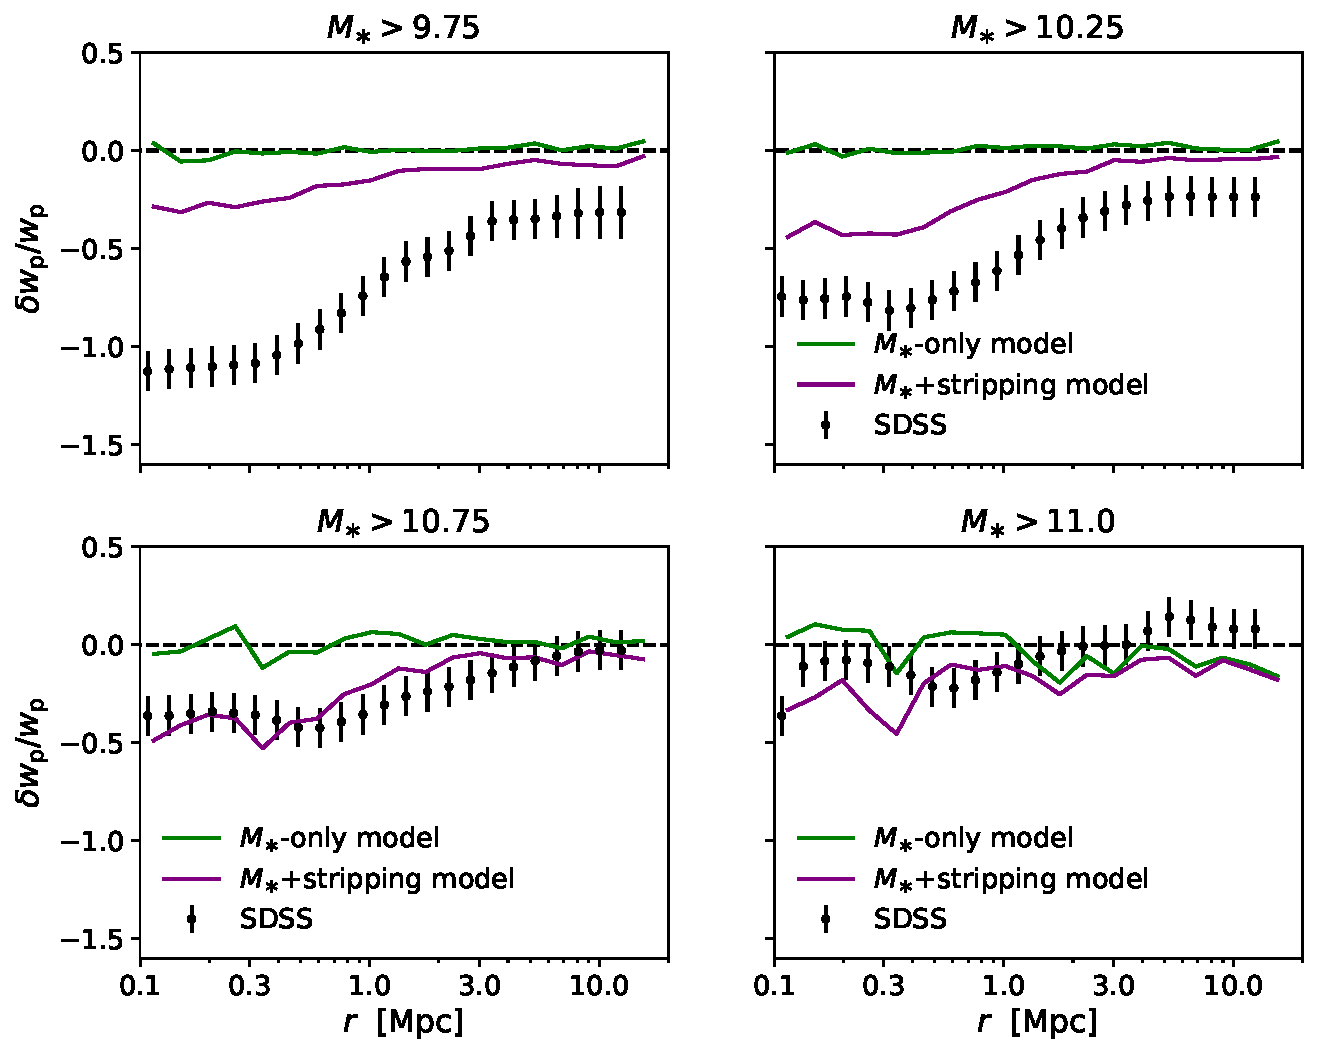
\includegraphics[width=8cm]{FIGS/alt_model_wp_ratios.pdf}
\caption{
{\bf Impact of tidal stripping.}
In all panels, the axes and points with error bars are the same as in Figure \ref{fig:clustering_ratio_upshot}. The solid green curves shows the prediction of the $\mstar-$based model, which is in gross tension with the data due to satellites having the same size as centrals of the same mass. The solid purple curves show results for a model in which satellites lose mass after infall in a manner similar to what is seen in high-resolution hydrodynamical simulations, as described in \S\ref{subsubsec:strippingmodel}. This produces satellites that are smaller than centrals, but the effect is too mild to correctly capture the observed clustering. Evidently, satellite-specific mass stripping plays a sub-dominant role in setting the relative size of centrals and satellites.
}
\label{fig:mstarmodelclustering}
\end{figure}
%-----------------------------------------------------------------------------------------------------


\subsection{The Role of Morphology and Color}
\label{subsec:colormorph}

In this section we take a preliminary look at how galaxy clustering exhibits simultaneous dependence upon broadband color, morphology, and size. Beginning from the $\mstar>10^{10.25}\msun$ sample used above, we first divide the sample into ``red" and ``blue" subsamples according to a $g-r=0.65$ cut, the rough location of the trough of the green valley for this stellar mass. For each color-selected subsample, we separately measure $\median{\rhalf}{\mstar; {\rm red}}$ and $\median{\rhalf}{\mstar; {\rm blue}},$ and use these median size values to split each subsample into two. 

In the top left panel of Figure \ref{fig:colorclustering} we show the clustering of large vs. small red galaxies; in the top right panel we show the same for blue galaxies. For each color-selected sample, large galaxies are slightly more strongly clustered relative to small galaxies. Comparing the top panels of Figure \ref{fig:colorclustering} to the the upper right panel of Figure \ref{fig:rvir_only_clustering_absolute} shows the dramatic impact of galaxy color selection upon $\rhalf-$dependent clustering. For $\mstar-$complete samples, small galaxies cluster much stronger than large galaxies; for color-selected samples, the reverse is true, and the magnitude of the effect weakens considerably.

The bottom panels of Figure \ref{fig:colorclustering} show results that are analogous to the top panels, but instead using of $g-r$ color, we first divide the $\mstar>10^{10.25}\msun$ sample into ``bulge-dominated" and ``disk-dominated" sequences according to $B/T,$ the fraction of $r-$band flux coming from the bulge component of the 2d light profile measurements in the \citet{meert_etal15} catalog. We define a galaxy as bulge-dominated if $B/T<0.25,$ and disk-dominated if $B/T>0.75.$ We separately split the disk-dominated and bulge-dominated subsample into two based on the median size $\median{\rhalf}{\mstar;B/T}$ appropriate for each subsample. The bottom left panel of Figure \ref{fig:colorclustering} compares the clustering of small vs. large disk-dominated galaxies; the bottom right panel shows the same comparison for bulge-dominated galaxies. 

The contrast between the two bottom panels is stark. The clustering of large vs. small bulge-dominated galaxies has almost no dependence upon $\rhalf.$ On the other hand, for disk-dominated galaxies, small galaxies are much more strongly clustered, and the effect is strong. In fact, comparing the bottom left panel of Figure \ref{fig:colorclustering} to the top right panel of Figure \ref{fig:rvir_only_clustering_absolute}, we see that $\rhalf-$dependent clustering is quite similar between disk-dominated galaxies and $\mstar-$threshold samples. We discuss a halo model interpretation of these trends in \S\ref{subsec:future}. 

The $\rhalf-$dependence of galaxy lensing has recently been measured using CFHTLenS observations \citep{heymans_etal12,erben_etal13}. For both red- and blue-sequence galaxies, it was found in \citet{charlton_etal17} that the lensing signal, $\Delta\Sigma,$ of large galaxies is slightly stronger relative to smaller galaxies. This result is in good agreement with the clustering measurements in the top panels of Figure \ref{fig:colorclustering}, which show the same trend. To date, the $\rhalf-$dependence of $\Delta\Sigma$ not yet been measured for $\mstar-$complete samples. We show  predictions of the $\rvir-$based model for future measurements of this signal in Figure \ref{fig:lensingprediction}. The halo model explanation for this trend is the same as for $\wproj:$ satellites occupy higher mass host halos relative to centrals of the same stellar mass, boosting $\Delta\Sigma$ for small relative to large galaxy samples. 

%---------------------------------------------------------------------------------------------------
\begin{figure*}
\centering
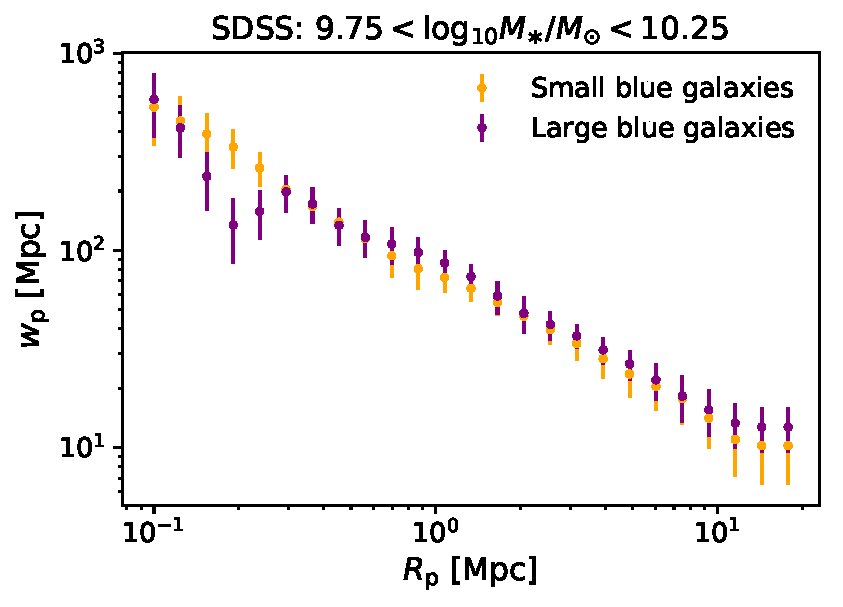
\includegraphics[width=8cm]{FIGS/blue_sdss_size_dependent_clustering_9p75_to_10p25.pdf}
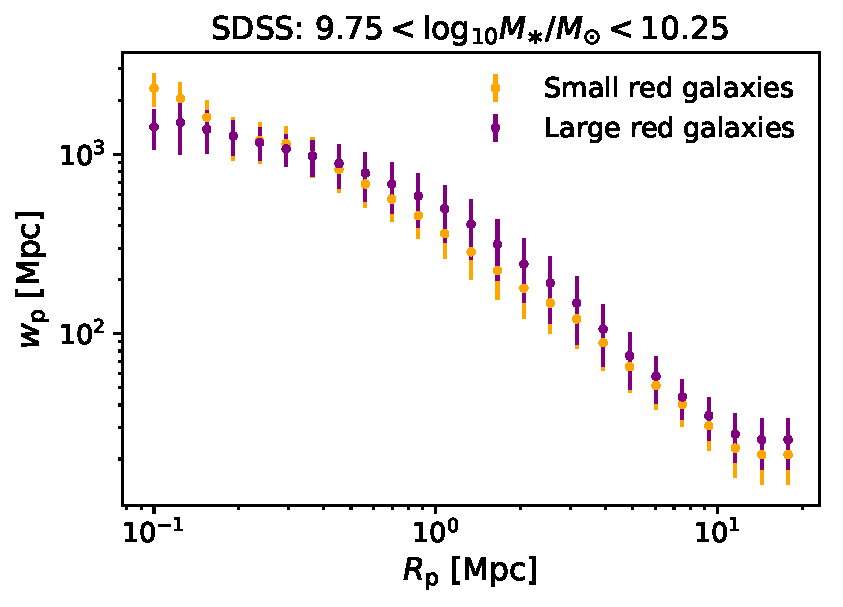
\includegraphics[width=8cm]{FIGS/red_sdss_size_dependent_clustering_9p75_to_10p25.pdf}
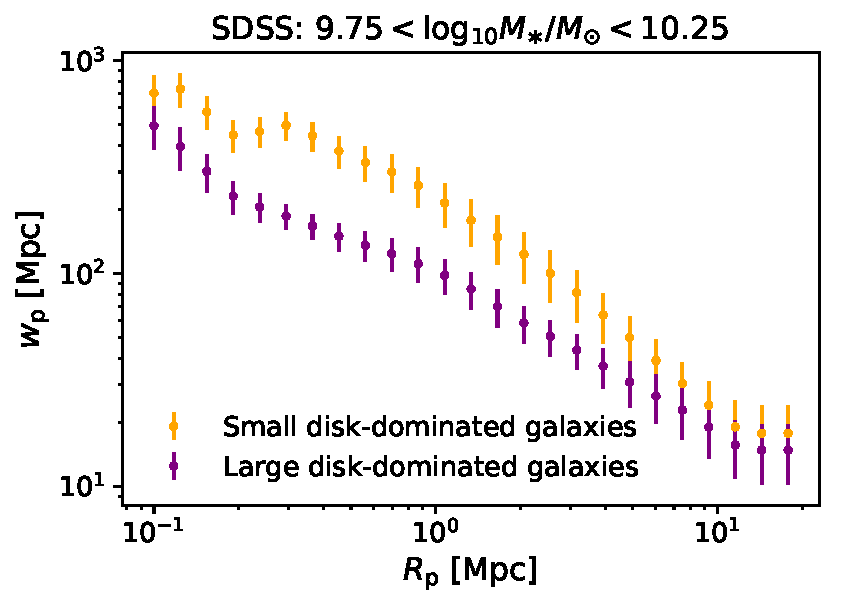
\includegraphics[width=8cm]{FIGS/disk_sdss_size_dependent_clustering_9p75_to_10p25.pdf}
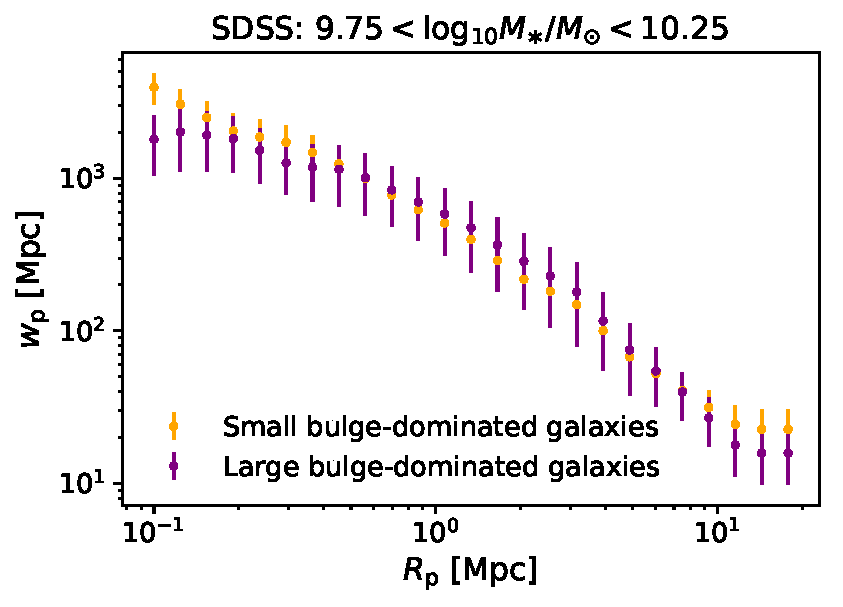
\includegraphics[width=8cm]{FIGS/bulge_sdss_size_dependent_clustering_9p75_to_10p25.pdf}
\caption{
{\bf Distinct $\rhalf-$dependence of clustering for color- or morphology-selected galaxy samples.}
All panels show the clustering of galaxies in the same bin of stellar mass: $10^{9.75}<\mstar/\msun<10^{10.25}.$ In the {\em upper left} panel, we first select blue galaxies based on $g-r<0.6,$ and subsequently compute $\median{\rhalf}{\mstar}$ {\em of the color-selected sample}. This results in identical stellar mass function for large and small blue galaxy samples, in analogy to the left panel of Figure \ref{fig:sizedefinition}. The {\em upper right panel} shows results of the same procedure for ``red" galaxies, defined by $g-r>0.6.$ The top two panels show that for color-selected samples, the magnitude of the $\rhalf-$dependence of clustering is dramatically reduced, and changes sign, relative to $\mstar-$complete samples. Using the \citet{meert_etal15} measurements of the disk/bulge decomposition of the 2d $r-$band luminosity profile $L_{\rm r},$ the bottom left panel shows analogous results for disk-dominated galaxies defined by $L_{\rm r}^{\rm bulge}<L_{\rm r}^{\rm tot}/4;$ the bottom right panel shows results for bulge-dominated galaxies defined by $L_{\rm r}^{\rm disk}<L_{\rm r}^{\rm tot}/4.$
}
\label{fig:colorclustering}
\end{figure*}
%---------------------------------------------------------------------------------------------------

%---------------------------------------------------------------------------------------------------
\begin{figure}
\centering
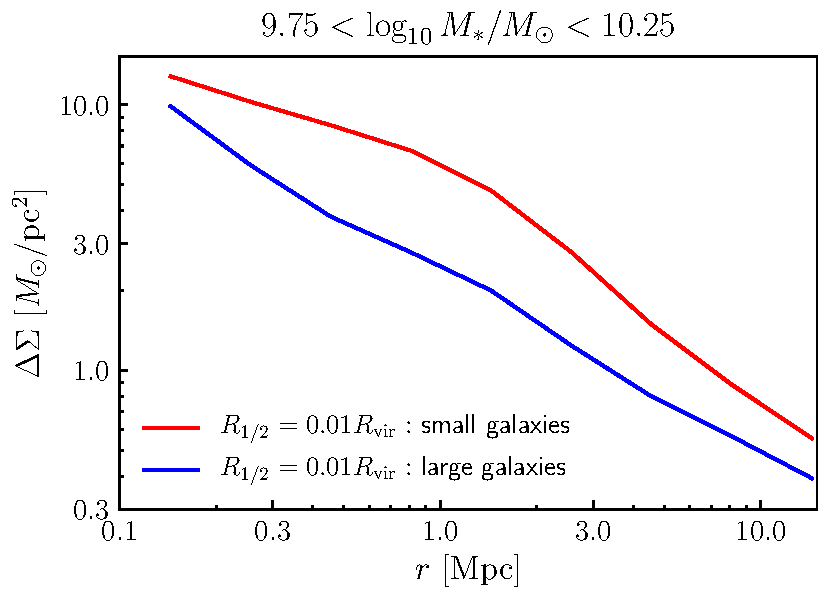
\includegraphics[width=8cm]{FIGS/rvir_only_lensing_prediction.pdf}
\caption{
{\bf Prediction for $\rhalf-$dependence of galaxy lensing.}
Using the $\rvir-$based model described in \S\ref{subsubsec:rvirmodel}, we make predictions for as-yet-unseen measurements of the $\rhalf-$dependence of galaxy lensing of $\mstar-$complete samples. To date, the $\rhalf-$dependence of $\Delta\Sigma$ has only been measured for color-selected samples \citep{charlton_etal17}, in which the reverse is true: for both blue and red samples, $\Delta\Sigma$ of small galaxies is (weakly) suppressed relative to large galaxies. As a generic consequence of satellites being smaller than centrals of the same mass, we predict that the analogous measurement for $\mstar-$complete samples will show $\Delta\Sigma$ of small galaxies to be much stronger relative to large galaxies of the same stellar mass.
}
\label{fig:lensingprediction}
\end{figure}
%-----------------------------------------------------------------------------------------------------

\section{Discussion}
\label{sec:discussion}

\subsection{Progression from Backwards to Forward Modeling}
\label{subsec:forwardsmodeling}

Our results give an archetypal demonstration of the natural scientific progression from backwards to forward modeling. In backwards modeling, some mapping is applied to observed galaxies to estimate the values of model quantities such as halo mass. In \citet{kravtsov13}, the model quantities mapped onto galaxies are $\mhalo$ and $\rvir;$ another classic example of backwards modeling uses a group- or cluster-finding algorithm to assign $\mhalo$ to observed galaxies \citep[e.g.,][]{berlind_etal06,yang_etal05a,rykoff_etal14}. Once the observed galaxies have been supplemented with model variables, then the relations of the galaxy-halo connection can be inferred, for example, by calculating quantities such as the mean stellar mass or quiescent fraction as a function of halo mass \citep[e.g.,][]{yang_etal05b,weinmann_etal06}.

In forward modeling, the direction of inference is turned around: a mapping is instead applied to the model quantities such as $\mhalo.$ In the case of {\tt Halotools}, this transforms a cosmological simulation into a synthetic galaxy catalog that can be directly compared with observations. This enables a richer quantitative study of modeling hypotheses relative to backwards modeling. For example, Figure \ref{fig:clustering_ratio_upshot} shows how forward modeling allows us to exploit galaxy clustering measurements to quantitatively test whether $\mhalo$ or $\mstar$ is the statistical regulator of galaxy size. The ability disentangle coupled variables such as $\mstar$ and $\mhalo$ is just one example of this advantage of forward modeling. Another example is illustrated in Figure \ref{fig:censatsizehist}, in which we explore the role of splashback halos in setting galaxy size. In our forward modeling approach, this is entirely straightforward; in backwards modeling, such an investigation would not even be possible without introducing additional modeling ingredients.

Backwards modeling the galaxy-halo connection is useful for generating hypotheses and motivating functional forms. Forward modeling becomes necessary when the problem at hand becomes encumbered by multiple relevant variables, as is the case with galaxy size. Forward modeling also makes it possible to conduct rigorous Bayesian inference, which we consider to be the next natural step in the progression described here (see \S\ref{subsec:future} for further discussion).

\subsection{Relation to Previous Work}
\label{subsec:previous_work}

Backwards modeling methods have been used extensively in the literature to gain insight into the relationship between galaxy mass, size, and environment. Broadly speaking, such studies proceed by using a galaxy group catalog to classify observed galaxies as centrals or satellites, and estimate their halo mass.  Employing such methods, several analyses of the \citet{yang_etal05b} group catalog have found that the $\mstar-\rhalf$ relation of early-type galaxies exhibits weak, if any, environmental dependence \citep{huertas_company_etal13b,shankar_etal14}.

A direct comparison to this finding is not possible because the conclusions drawn here pertain to $\mstar-$limited galaxy samples. As discussed in \citet{spindler_wake17}, it is entirely possible that size differences between centrals and satellites of the same mass can be accounted for by mutual covariance with an additional variable such as star formation rate or morphological type \citep[see also][for an explicit demonstration of this scenario]{lilly_carollo16}. In particular, suppose that centrals and satellites of the same mass have different early-type fractions as indicated in \citet{weinmann_etal06}, and that early- and late-type galaxies exhibit universal, but distinct, $\mstar-\rhalf$ relations. In such a case, centrals would be larger than satellites of the same mass, even though {\em early-type centrals} would have the same sizes as {\em early-type satellites}.

As discussed in \S\ref{subsec:future}, we are currently pursuing follow-up work in which we jointly model morphological type together with galaxy size. We consider forward modeling methods to be a requisite for progress on this issue, not only to properly handle the multi-dimensional nature of the problem, but also to rigorously treat systematic errors that plague inference based on galaxy group catalogs \citep[see][for a thorough discussion]{campbell_etal15}.

Our approach is closely aligned with the methods used in \citet{somerville_etal17}, who studied the empirical modeling features that are necessary to recover the tight scatter in the observed $\langle\rhalf\vert\mstar\rangle$ relation. By building models where $\rhalf$ is set by halo spin $\lambda_{\rm halo}$, the authors in \citet{somerville_etal17} found that the level of intrinsic scatter about $\langle\lambda_{\rm halo}\vert\mhalo\rangle$ in dark matter halos is at least as large as the scatter about $\langle\rhalf\vert\mstar\rangle$ seen in observed galaxies. Since the latter necessarily receives an additional contribution from measurement error, this implies some tension with the common semi-analytic modeling assumption that $\lambda_{\rm halo}$ scales with $\rhalf.$ As noted in \citet{somerville_etal17}, tension in the level of scatter cannot be used to directly test the $\lambda_{\rm halo}\propto\rhalf$ assumption because the physical motivation for this correlation is largely limited to disk galaxies \citep{mo_mao_white98}. This tension is not present in our approach for the reason that the level of scatter is simply a modeling parameter in our approach, and we make no attempt to uncover the physical origin of this scatter. However, our fiducial value choice was motivated by \citet{somerville_etal17}, and in the ongoing follow-up work discussed in \S\ref{subsec:future} we will systematically test the large-scale structure implications of the assumption that $\lambda_{\rm halo}\propto\rhalf^{\rm disk}.$

\subsection{Implications for Satellite Evolution}
\label{subsec:satellite_discussion}

Our treatment of satellite-specific mass loss with the $\mstar+$stripping model is only approximate, because we have  modified the size of satellites without self-consistently modifiying their total stellar mass. In the present work, we have opted not to develop and fine-tune a more complex, semi-analytic model; instead, we have made a simple estimate for the level at which satellite-specific stripping impacts the two-point function.

%Explanations for differences between the sizes of centrals and satellites fall into two categories, depending on whether or not the processes involved are specific to post-infall physics. One obvious possibility that could lead to satellites being smaller than centrals of the same $\mhalo$ is tidal stripping: satellite $\mstar$ could decrease after infall, reducing the size of the galaxy. We have quantitatively tested this possibility with the $\mstar-$stripping model described in \S\ref{subsubsec:strippingmodel}. Comparing the clustering ratios of the ``$\rvir-$based" and ``$\rvir+$stripping" models in Figure \ref{fig:strippingorphans}, we find that the impact of physically motivated levels of satellite mass loss cannot explain the $\rhalf-$dependent clustering seen in SDSS. As an additional test, we reach the same conclusion when implementing an even more extreme $\mstar-$stripping model in which stellar mass loss is linearly proportional to halo mass loss \citep[][Model 1]{watson_etal12}.

%Both the $\rvir-$based model and the co-evolution model (see sections \S\ref{subsubsec:rvirmodel} and \S\ref{subsubsec:coevolutionmodel}, respectively) represent explanations falling into the second category, in which centrals and satellites of the same $\mhalo$ have different sizes due to their different evolutionary paths {\em prior} to satellite infall. For these models the story is very different: the influence of pre-infall co-evolution has a dramatic impact on $\rhalf-$clustering ratios, with a scale- and $\mstar-$dependence that closely resembles the SDSS signal. Quantitative constraints on the true level of this co-evolution effect will be a natural outcome of the program described in \S\ref{subsec:future}, but it is already clear that the long term co-evolution of galaxy and halo profiles should be considered a critical ingredient to models for the distribution of galaxy sizes across the cosmic web.

\subsection{Future Directions for Empirical Modeling of Galaxy Size}
\label{subsec:future}

\subsubsection{Jointly modeling $\langle\mstar\vert\mhalo\rangle$}

%The scope of this work is to serve as a pilot study in which we identify the chief ingredients that can influence the $\rhalf-$dependence of galaxy clustering. While our results suggest that our profile co-evolution model is giving the correct qualitative picture, our implementation cannot be correct in quantitative detail: the clustering ratios of this model shown in Figure \ref{fig:clustering_ratio_upshot} are too strong relative to SDSS. This likely indicates that the central/satellite size differences depicted in Figure \ref{fig:} are too strong, and that the correlation strength in the real Universe is intermediate, rather than maximal. Our publicly available code that reproduces our results already contains the machinery to implement continuously variable levels of $\rhalf-\rspeak$ correlation strength, but for present purposes we have chosen to focus on exploring bracketing cases of qualitative ingredients, rather than fine-tuning the model.

%In addition to varying the $\rhalf-\rspeak$ correlation strength, there are other factors that should be included in any proper likelihood analysis of galaxy size models. In particular, since the clustering signal is strongly influenced by differences between centrals and satellites, then the satellite fraction $F_{\rm sat}(\mstar)$ plays an important role in $\rhalf-$dependent clustering. For fixed scaling relations $\langle\rhalf^{\rm cens}\vert\mhalo\rangle$ and $\langle\rhalf^{\rm sats}\vert\mhalo\rangle,$ models with different satellite fractions will exhibit different $\rhalf-$clustering ratios because $F_{\rm sat}(\mstar)$ controls the relative weighting of the two populations. Our results based on the catalog that includes orphan subhalos (Figure \ref{fig:strippingorphans}, dotted curves) give an explicit demonstration of the impact of $F_{\rm sat}(\mstar)$ on the clustering signal.

%On the one hand, this degeneracy with the satellite fraction is unfortunate, because it means galaxy sizes does not leave a pure and unique signature on $\rhalf-$clustering ratios. However, this can also be viewed as an opportunity to extract tighter constraints on $F_{\rm sat}(\mstar),$ which are sorely needed to discriminate between competing models. For this problem, the path forward is clear. Traditional galaxy clustering is already being used to validate and/or fit models of the stellar-to-halo-mass relation \citep[e.g.,][]{moster_etal13,behroozi13_smhm,lehmann_etal15}. Based on our results, we advocate that empirical models for $\langle\mstar\vert\mhalo\rangle$ be supplemented with additional model ingredients for $\langle\rhalf\vert\mstar\rangle,$ and that the parameters of composite model are jointly constrained by measurements of the stellar mass function, $\mstar-$dependent clustering, and $\rhalf-$dependent clustering. Careful attention will need to be paid to the orphan subhalo population, which is well-known to have a significant impact on small-scale clustering \citep{guo_white13,campbell_etal17}.

\subsubsection{Jointly modeling morphology}

A proper interpretation of the results clustering results shown in Figure \ref{fig:colorclustering} requires forward-modeling the joint dependence of the galaxy-halo connection upon $\mstar, \rhalf, g-r, $ and $B/T,$ which is beyond the scope of this work. Nonetheless, the broad features of these $\wproj(\rproj)$ measurements give insight into the characteristics that any model for these properties should exhibit. 

First, the bottom right panel of Figure \ref{fig:colorclustering} indicates that the size of the bulge has only a tenuous connection to the properties of its parent dark matter halo.\footnote{Strictly speaking, the size of the bulge could in principle be closely connected to any number of dark matter halo properties, so long as those halo properties do not significantly impact two-point clustering.} Second, for disk-dominated galaxies, the observed $\rhalf-$dependent clustering suggests that at fixed $\mstar,$ the size of the disk is strongly correlated with whether or not the galaxy is a satellite. 

%Previous studies of large-scale structure measured by SDSS indicate that morphological type has a significant influence on galaxy clustering \citep{skibba_etal08}. Because morphology is covariant with star-formation rate (SFR) and $\rhalf,$ accounting for this dependency will require simultaneously modeling each of these variables.

%To date, such a task has been beyond the purview of empirical models. However, recent progress has substantially improved the richness of the predictions that galaxy-halo models are capable of \citep{becker15,cohn17,moster_etal17}. This new class of models has accomplished this by empirically modeling star-formation rate, and then integrating SFR along each halo's history to differentially build up stellar mass.\footnote{This approach towards predicting $\mstar$ is thus mathematically akin to traditional semi-analytic models, although \citet{becker15} have retained the empirical modeling prioritization of simplicity and computational efficiency.} We are currently extending this new class of models to differentially build up the disk and bulge across cosmic time. In addition to treating the multi-dimensional nature of the problem, this also allows us to use data at higher redshift in a self-consistent manner.


\section{Conclusions}
\label{sec:conclusion}

We have presented new measurements of the dependence of galaxy clustering upon galaxy size, and used {\tt Halotools} to identify the basic ingredients that influence the signal. We conclude with a brief summary of our primary findings:

\ben
\item Small galaxies cluster more strongly than large galaxies of the same stellar mass. Differences between the clustering of small and large galaxies increase on small scales $R\lesssim1\mpc,$ and decrease with stellar mass.
\item The most important ingredient influencing this signal is the relative size of central and satellite galaxies. The magnitude, scale-dependence, and $\mstar-$dependence of $\rhalf-$dependent clustering provides strong evidence that satellite galaxies are smaller than central galaxies of the same halo mass.
\item A simple empirical model in which $\rhalf$ is set by halo $\rvir$ at the time of peak halo mass exhibits a clustering signal that is strikingly similar to that seen in SDSS.
\item Models in which $\rhalf$ is regulated by $\mstar,$ rather than $\mhalo,$ are grossly discrepant with the observed clustering signal, even when accounting for satellite mass stripping.
\item Taken together, our findings indicate that satellite-specific processes play a sub-dominant role in setting the relative size of centrals and satellites, which instead appears to be largely predetermined at the time of satellite infall.
\een

Our results can be treated as a boundary condition for more complex and fine-grained models of galaxy size, such as semi-analytic models and hydrodynamical simulations. We view the present work as a pilot study that motivates a Bayesian inference program to tightly constrain the galaxy size-halo connection with forward modeling techniques, in direct analogy to the literature on the stellar-to-halo-mass relation. Our publicly available python code provides a simple means for cosmological surveys to generate synthetic galaxy populations with realistic sizes across the cosmic web.

\section*{Acknowledgments}

APH thanks John Baker for the {\em Toejam \& Earl} soundtrack. Thanks also to Frank van den Bosch, Doug Watson, and Risa Wechsler for thoughtful feedback at various stages of the development of this work, and to Faustin Carter and Sebastian Bocquet for sharing their python expertise.

We thank the {\tt Astropy} developers for the package-template \citep{astropy}, and {\tt NumPy} \citep{numpy_ndarray}, {\tt SciPy} \citep{scipy}, IPython, Matplotlib, and GitHub for their extremely useful free software.

This research was supported in part by the National Science Foundation under Grant No. NSF PHY11-25915. Work done at Argonne National Laboratory was supported under the DOE contract DE-AC02-06CH11357.

\bibliography{galsize_paper}

\section*{Appendix: Treatment of Disrupted Subhalos}

We use an extension of {\tt Consistent Trees} that models the evolution of subhalos after disruption. The phase space evolution of disrupted subhalos is approximated by following a point mass evolving in the host halo potential according to the orbital parameters of the subhalo at the time of disruption; the evolution of subhalo mass and circular velocity is approximated using the semi-analytic model presented in \citet{jiang_vdB14}. We then use the {\tt orphans} program in {\tt UniverseMachine} to walk through all the Bolshoi-Planck {\tt hlist} files, yielding the main progenitor information of every subhalo that was ever identified by {\tt Consistent Trees}.

Since it is likely that some portion of these disrupted subhalos should be populated with model galaxies \citep{guo_white13, campbell_etal17}, in our initial application of deconvolution abundance matching we derive the $\mstar--\mpeak$ relation using {\em all} subhalos, including those that may be disrupted. We then apply a selection function to the disrupted subhalos, so that a fraction of these objects will host galaxies in our mock universe. We refer to this as the {\em orphan selection function}, $\mathcal{F}_{\rm orphan},$ which we consider to be an integral component of our application of abundance matching.

Since a rigorous calibration of $\mathcal{F}_{\rm orphan}$ is beyond the scope of the present work, we instead opt for a simple parameterization that yields reasonably accurate recovery of the galaxy clustering signal observed in SDSS. We model $\mathcal{F}_{\rm orphan}=\mathcal{F}_{\rm orphan}(M_{\rm peak},M_{\rm host}),$ where $\mpeak$ is the peak mass of the disrupted subhalo, and $\mhost$ is the present-day virial mass of its $z=0$ host halo. For the $\mpeak-$dependence, we select $50\%$ of disrupted subhalos with $\mpeak=10^{11}\msun,$ $0\%$ of subhalos with $\mpeak=10^{13}\msun,$ linearly interpolating in $\log\mpeak$ for intermediate values of $\mpeak.$ At each $\mpeak,$ the selection of disrupted halos is not random; instead, we preferentially select the subhalos with larger $\mhost,$ which we intend to offset the increased difficulty of subhalo-finding algorithms to identify subhalos with especially small values of  $\mu\equiv\mpeak/\mhost.$

%As the orphan catalog has a higher satellite fraction than the standard subhalo catalog, the negative boost shown the dotted curves in Figure \ref{fig:strippingorphans} is expected. Orphan halos also typically have earlier-than-average values of $\zpeak$ relative to ordinary subhalos, which also enhances differences between central and satellite sizes. See \S\ref{subsec:satellite_discussion} for further discussion.

\end{document}







